% %!TEX root = main.tex
\subsection{The Internet of Things}


\begin{frame}
\frametitle{IoT definition}
The Internet of Things is <insert preferred definition>.
\end{frame}


\begin{frame}
\frametitle{IoT definition}
The Internet of Things is a generalization of the World Wide Web to incorporate ``things'' that exist in the physical world. 
\end{frame}

\begin{frame}
\frametitle{IoT definition}
The Internet of Things is the convergence of all virtual and physical entities that are able to produce, consume and act upon data under a common communications infrastructure.
\end{frame}

\begin{frame}
\frametitle{Synaisthisi Platform}
The Synaisthisi platform is a project developed in NCSR Demokritos that aims to facilitate the development of Internet of Things applications.

It provides
\begin{itemize}
\item A \textbf{Service Oriented Architecture} where applications can be developed as the composition of small functional building blocks (services) 
\item A categorization of services in Sensing, Processing and Actuating (\textbf{SPA services})
\item A \textbf{Message Oriented Middleware} that provides a pub/sub message passing infrastructure based on MQTT for inter-service communication
\item Mechanisms for logging, security, persistent storage, data replication and administration of the applications and the system
\end{itemize}
\end{frame}


\begin{frame}
\frametitle{Synaisthisi Architecture}

\begin{figure}[!htb]
\centering
\resizebox{0.85\linewidth}{!}{
	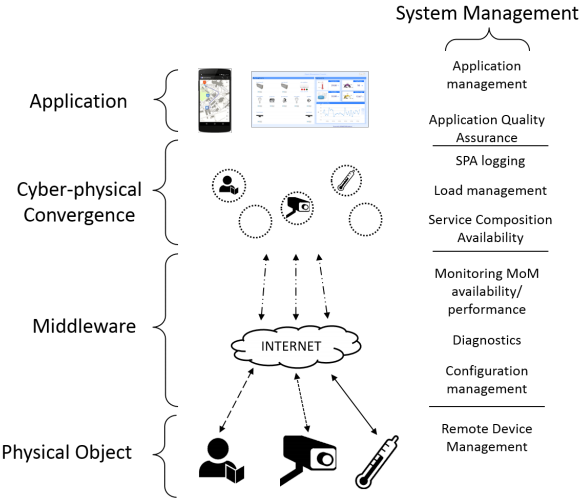
\includegraphics[]{figs/synaisthisi-arch}
}
\end{figure}

\end{frame}